\section{OPQ Architecture}
\label{sec:architecture}

\subsection{System Architecture}

At its most basic, the OPQ system architecture is this: OPQ Boxes are plugged into wall outlets, they monitor the quality of power at their wall outlets, and the results are communicated via the Internet to a software system called OPQ Cloud. To see the results, users login to the system using a browser.

A slightly less basic description is this: the OPQ system architecture consists of four major open source hardware and software components that provide end-to-end support for the capture, triggering, analysis, and reporting of consumer level local and global PQ events:

\begin{enumerate}

\item OPQ Box is a hardware device that detects the electrical waveform from a standard residential outlet and communicates both low and high fidelity representations of the waveform to other OPQ system components either at predefined intervals or upon request.

\item OPQ Makai monitors incoming low fidelity data from OPQ Boxes, requests high fidelity data when necessary, and stores the results in a MongoDB database.

\item OPQ Mauka analyzes low level data and analyzes it to produce higher-level representations according to the information architecture described below, and can tell OPQ Makai to request high fidelity data from one or more OPQ Boxes to facilitate analysis.

\item OPQ View is a browser-based visualization platform for displaying the results for data capture and analysis.

\end{enumerate}

\begin{figure}
\center 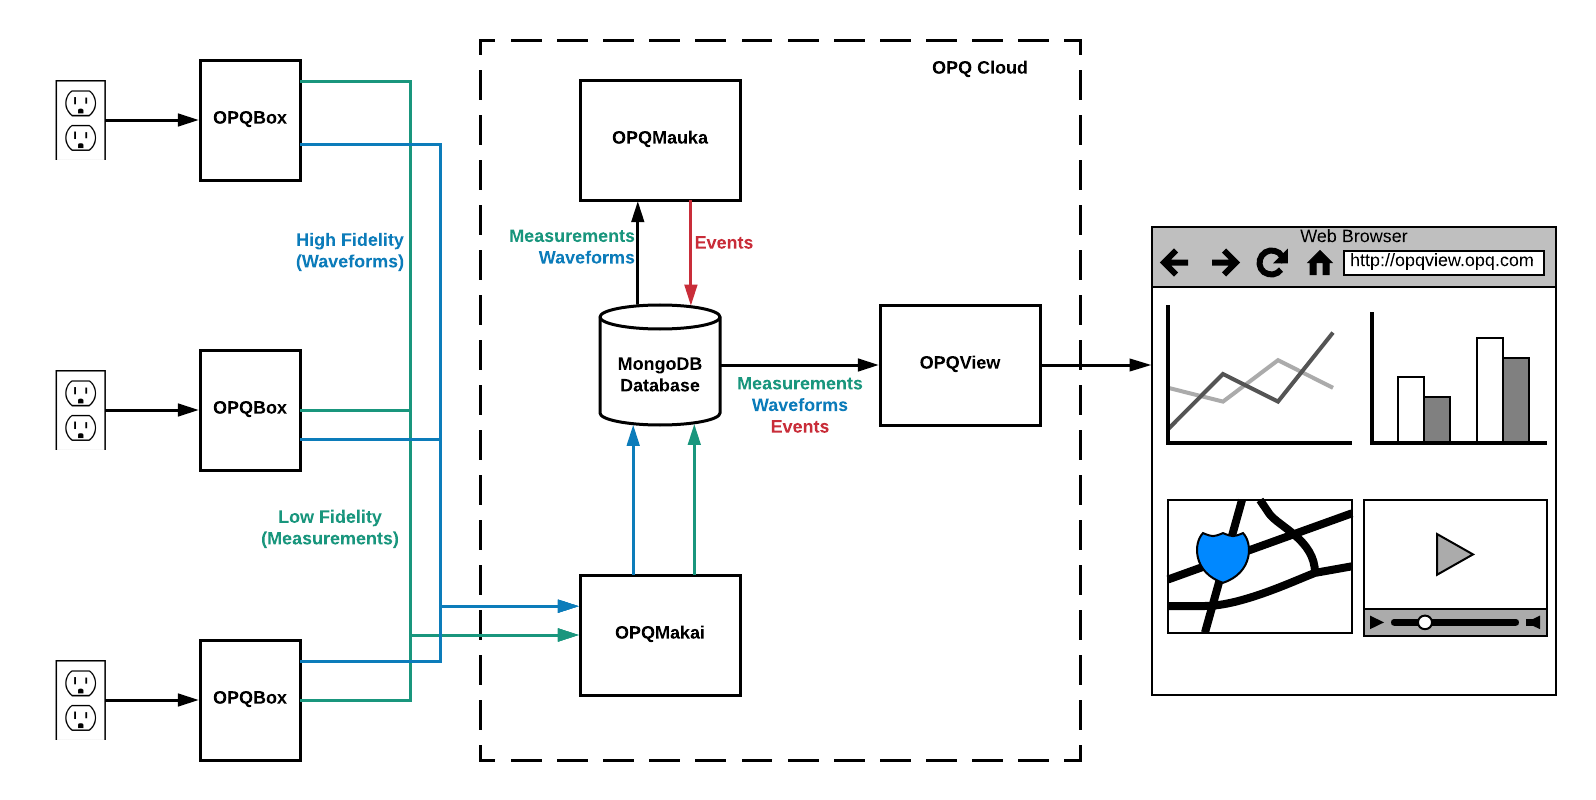
\includegraphics[width=5in]{images/architecture/system-diagram.png}
\caption{High level system architecture of an OPQ Sensor Network}
\label{fig:architecture}
\end{figure}


Figure \ref{fig:architecture} illustrates how these components work together to take information from wall outlets (on the left side) to the display of analyses in a browser (on the right hand side).  First, OPQ Boxes analyze power from wall outlets, and send low fidelity measurements to OPQ Makai. OPQ Makai analyzes low fidelity measurements, and requests high fidelity waveforms when desirable. Both measurements and waveforms are saved in a MongoDB database. OPQ Mauka analyzes low and high fidelity data, and creates "events" to represent anomalies. OPQ View notifies users of events and allows them to drill down into low and high fidelity data.

OPQ Makai, OPQ Mauka, and OPQ View are all cloud-based software services that collectively form a single "instance" with respect to data transmission, storage, analysis, and visualization. We refer to this collection of software-side components as OPQ Cloud. Every OPQ Box connects to a single instance of an OPQ Cloud. It is possible to have multiple OPQ Cloud instances. For example, a company might install an OPQ Cloud instance behind their firewall along with OPQ Boxes to provide a private mechanism for collecting and analyzing power quality data.

This architecture has a number of benefits. The combination of low and high fidelity data reduces both network overhead and storage requirements, which increases the scalability of the system in terms of the number of OPQ Boxes that can be tied to a single OPQ Cloud instance. OPQ Makai and OPQ Mauka have a plugin architecture, making it easier to extend their functionality to incorporate new triggers for high quality data (in the case of OPQ Makai) and new events and power analyses (in the case of OPQ Mauka). Finally, the open source licensing of both hardware and software makes it possible to incorporate new ideas, bug fixes, and enhancements from technologists across the power quality community.

\subsection{Information Architecture}

OPQ's "information architecture" is designed to facilitate the process of generating actionable, useful insights into the nature of the electrical grid starting with the data collected from a wall outlet. The information architecture must address several requirements. First, it must support analyses that require access to high fidelity data, which in the case of power quality is wave form data produced by sampling the wave form 256 times per cycle (or 12,000 times per second), which means there are approximately 1 billion data points generated per day per OPQ Box. Second, for typical grids that are generally stable, only an extremely small fraction of these data points are actually interesting. Third, as will be discussed in more detail later, what constitutes ``interesting'' data in one box might be dependent upon the state of data in other nearby boxes. Finally, network and storage limitations preclude a solution in which all data is sent from OPQ Boxes to the cloud, and so the information architecture must provide a ``smart'' mechanism for identifying data of interest on the boxes, as well as discarding data in the cloud if it is found to be not useful.

To address these requirements, the OPQ information architecture is organized as a five layer pyramid as summarized in Table \ref{fig:information-architecture}. This table illustrates an important conceptual feature of the OPQ information architecture called ``TTL'', or Time To Live. The OPQ information architecture implements an active, ``use it or lose it'' approach to information management, in which a data item must either be associated with a higher level of the system within its Time To Live, or else it will be automatically deleted. So, for example, the high fidelity waveform data on an OPQ Box have a TTL of one hour: if that data is not requested from a box by a higher layer in the information architecture within an hour of it being generated, it will be lost. Similarly, data points in the Measurement layer will be deleted after one day if they are not associated with an Event.

\begin{table}[ht]
\caption{OPQ Information Architecture Levels}
\centering
%% \tablesize{} %% You can specify the fontsize here, e.g., \tablesize{\footnotesize}. If commented out \small will be used.
\begin{tabular}{llp{4in}}
\toprule
\textbf{Layer}	& \textbf{TTL}	& \textbf{Purpose}\\
\midrule
Box		& 1 hour			& Collects and holds a rolling one hour window of "high fidelity" instantaneous wave form data measurements for a single location.\\
Measurement		& 1 day/2 weeks		& Aggregate measurements provide "low fidelity" summary statistics regarding four power measurements (Frequency, Voltage, THD, Transients) at a rate of either 1/second (Measurement) or 1/day (Trend). Measurements and Trends both collect summary statistics, but at different window lengths and with different TTLs.\\
Event/Detection & 1 month & When OPQ Cloud's Makai service detects non-nominal values in the stream of Measurements, it can decide to request an ``event'': wave form data from one or more boxes for a specific time interval (typically, just a second or so). \\
Incident & 6 months & An Incident is generated by OPQ Cloud's Mauka when an Event satisfies a standard (such as IEEE 1159, ITIC, or SEMA) for a significant power quality problem.\\
Phenomena & 1 year & Phenomena classify Incidents when they are predictable and/or have a known causal explanation. \\
\bottomrule
\end{tabular}
\label{fig:information-architecture}
\end{table}

Let's now discuss how information moves through these levels.

The bottom layer of the information architecture is called Box, and represents all of the OPQ Box hardware devices in an OPQ sensor network. Each box maintains onboard storage of the latest hour of high quality waveform data in a circular buffer.

Approximately once a second, each Box sends a Measurement data object to the sensor network's cloud services, which we refer to in aggregate as OPQ Cloud. Measurements are the second layer of the information architecture, and provide "low fidelity" summary statistics regarding four power quality measurements (Frequency, Voltage, THD, and Transients). Measurements give OPQ Cloud basic situational awareness of the grid without the overhead of transmitting, storing, and analyzing high fidelity wave form data. Measurements exist for one day, though a daily roll-up of Measurement summary statistics called "Trends" persists longer.

When OPQ Cloud's Makai service detects non-nominal values in the stream of Measurements, it can decide to request wave form data from one or more boxes for a specific time interval (typically just a second or so). Note that Makai only has one hour to request high fidelity wave form data before it is lost. Mauka may also request Event data for specific Phenomena, which will be discussed in more detail below.

Not every non-nominal power data value is significant, or in other words, meaningful for gaining insight into the grid. Over the years, the power community has developed a variety of standards (IEEE 1159, ITIC, SEMA, etc.) for characterizing significant power quality events. OPQ Cloud's Mauka service provides classification algorithms to analyze each Event to see if it satisfies any of the standards for significance. If so, an Incident is created, indicating that a significant PQ event has occurred at a specific time in a specific location. Each Incident can also be annotated with context, which is additional information about the environment or other physical factors present at the time and location of this incident. Context can be manually provided by users or automatically associated with Incidents through APIs to online services.

All of the prior levels represent behaviors of individual Boxes in a single location at a given point in time. This final level of OPQ's information architecture is premised on the idea that insightful, actionable information results from the ability to either explain or else predict multiple Incidents. First, a Phenomena can be created in order to collect data from multiple Incidents with a common cause. An example of this form of phenomena is "the voltage drop experienced by all boxes in Kailua on 5/22/18 at 1:03pm was caused by a transformer trip at the Kailua substation." Second, a Phenomena can collect data from multiple Incidents in order to predict future Incidents. For example, "when winds exceed 40 knots in Kahuku, data from prior Incidents leads to the prediction that there will be a voltage surge of approximately 5V for approximately 3 seconds in all boxes located within 1 mile of Kahuku."

Further details of this information hierarchy are provided in Section~\ref{sec:opq-mauka}.

